\documentclass[xetex,mathserif,serif]{beamer}

\usepackage{xunicode}
\usepackage{xltxtra}
\usepackage{color}
\usepackage{url}
\usepackage{listings}
\usepackage{fontspec}
\usepackage{geometry}
\usepackage{lastpage}
\usepackage{fancyhdr}
\usepackage{amsmath}
\usepackage{amsthm}
\usepackage{amssymb}
\usepackage{blkarray}
\usepackage{multicol}
\usepackage{relsize}

\definecolor{solarized@base03}{HTML}{002B36}
\definecolor{solarized@base02}{HTML}{073642}
\definecolor{solarized@base01}{HTML}{586e75}
\definecolor{solarized@base00}{HTML}{657b83}
\definecolor{solarized@base0}{HTML}{839496}
\definecolor{solarized@base1}{HTML}{93a1a1}
\definecolor{solarized@base2}{HTML}{EEE8D5}
\definecolor{solarized@base3}{HTML}{FDF6E3}
\definecolor{solarized@yellow}{HTML}{B58900}
\definecolor{solarized@orange}{HTML}{CB4B16}
\definecolor{solarized@red}{HTML}{DC322F}
\definecolor{solarized@magenta}{HTML}{D33682}
\definecolor{solarized@violet}{HTML}{6C71C4}
\definecolor{solarized@blue}{HTML}{268BD2}
\definecolor{solarized@cyan}{HTML}{2AA198}
\definecolor{solarized@green}{HTML}{859900}
\definecolor{yaleblue}{HTML}{0E4C92}

\setbeamertemplate{navigation symbols}{}
% \setbeamerfont{title}{family=\old}
% \setbeamerfont{author}{family=\tfont}%
% \setbeamerfont{frametitle}{family=\oldA}
% \setbeamerfont{date}{family=\dfont}

\setbeamertemplate{itemize items}{--}
\setbeamercolor*{item}{fg=black}

\defaultfontfeatures{Mapping=tex-text}
\hypersetup{pdfstartview={FitH}}

\newcommand{\old}[1]{\fontspec[Alternate=1,Ligatures={Common}]{Hoefler Text}\fontsize{18pt}{30pt}\selectfont #1}%
\newcommand{\oldA}[1]{\fontspec[Alternate=1,Ligatures={Common, Rare}]{Hoefler Text}\fontsize{12pt}{15pt}\selectfont #1}%
\newcommand{\oldB}[1]{\fontspec[Ligatures={Common}]{Didot}\fontsize{12pt}{15pt}\color{solarized@base02}\selectfont #1}%
\newcommand{\tfont}[1]{\fontspec[Alternate=1,Ligatures={Common}]{Hoefler Text}\fontsize{12pt}{20pt}\selectfont #1}%
\newcommand{\dfont}[1]{\fontspec[Ligatures={Common}]{Didot}\fontsize{12pt}{12pt}\selectfont #1}%

\newcommand{\minimize}{\mathop{\mathrm{minimize}}}
\newcommand{\argmin}{\mathop{\mathrm{arg\,min}}}
\newcommand{\argmax}{\mathop{\mathrm{arg\,max}}}
\newcommand{\st}{\mathop{\mathrm{subject\,\,to}}}

\newcommand\independent{\protect\mathpalette{\protect\independenT}{\perp}}
\def\independenT#1#2{\mathrel{\rlap{$#1#2$}\mkern2mu{#1#2}}}

\setlength{\parindent}{0pt}
\setlength{\parskip}{12pt}

\setromanfont [Ligatures={Common}, Numbers={OldStyle}, Variant=01,
 BoldFont={LinLibertine_RB.otf},
 ItalicFont={LinLibertine_RI.otf},
 BoldItalicFont={LinLibertine_RBI.otf}
 ]{LinLibertine_R.otf}



\begin{document}

%%%%%%%%%%%%%%%%%%%%%%%%%%%%%%%%%%%%%%%%%%%%%%%%%%%
\begin{frame}[fragile] \frametitle{}

\vfill

{\fontsize{0.7cm}{0cm}\selectfont Lecture 11 \\\vspace{0.2cm}
Weighted Least Squares and Review}\\\vspace{0.5cm}
07 October 2015

\vspace{2cm}

\begin{minipage}{0.6\textwidth}
Taylor B. Arnold \\
Yale Statistics \\
STAT 312/612
\end{minipage}
\hfill
\begin{minipage}{0.3\textwidth}\raggedleft

\includegraphics[scale=0.3]{../yale-logo.png}
\end{minipage}%

\end{frame}

%%%%%%%%%%%%%%%%%%%%%%%%%%%%%%%%%%%%%%%%%%%%%%%%%%%
\begin{frame}[fragile] \frametitle{}

{\color{yaleblue}\fontsize{16pt}{20pt}\selectfont Notes}

\begin{itemize}
\item Problem Set \#3 - Due today
\item Review session on Sunday, 4pm at 24 Hillhouse
\item Midtern I - In class, next Monday
\end{itemize}

\end{frame}

%%%%%%%%%%%%%%%%%%%%%%%%%%%%%%%%%%%%%%%%%%%%%%%%%%%
\begin{frame}[fragile] \frametitle{}

{\color{yaleblue}\fontsize{16pt}{20pt}\selectfont Goals for today}

\begin{itemize}
\item Notes on weighted least squares and GLS
\item Review of the standard linear regression theory
\end{itemize}

\end{frame}

%%%%%%%%%%%%%%%%%%%%%%%%%%%%%%%%%%%%%%%%%%%%%%%%%%%
\begin{frame}[fragile] \frametitle{}

\begin{flushright}
{\color{yaleblue}\sc\fontsize{1cm}{0cm}\selectfont WLS and GLS}
\end{flushright}

\end{frame}

%%%%%%%%%%%%%%%%%%%%%%%%%%%%%%%%%%%%%%%%%%%%%%%%%%%
\begin{frame}[fragile] \frametitle{}

On the problem set, you considered a regression model where the
covariance marix of the error terms is known to be proportional
to some matrix $V(X)$.

\end{frame}

%%%%%%%%%%%%%%%%%%%%%%%%%%%%%%%%%%%%%%%%%%%%%%%%%%%
\begin{frame}[fragile] \frametitle{}

The standard way to solve this
problem is to decompose the inverse of $V$ as $C^t C$, and to
left multiply the regression problem by $C$:
\begin{align*}
y &= X \beta + \epsilon \\
Cy &= C X \beta + C\epsilon \\
\tilde{y} &= \tilde{X} \beta + \tilde{\epsilon}
\end{align*}
\pause Now, we see that the covariance matrix of the transformed error
terms are spherical:
\begin{align*}
\mathbb{V} (\tilde{\epsilon} | X) &= \mathbb{E} (\tilde{\epsilon} \tilde{\epsilon}^t | X) \\
&= \mathbb{E} ( C \epsilon \epsilon^t C^t | X) \\
&= C \, \mathbb{E} ( \epsilon \epsilon^t | X) C^t \\
&= \sigma^2 C V C^t \\
&= \sigma^2 \mathbb{I}_n \\
\end{align*}

\end{frame}

%%%%%%%%%%%%%%%%%%%%%%%%%%%%%%%%%%%%%%%%%%%%%%%%%%%
\begin{frame}[fragile] \frametitle{}

The (very) important thing to notice about this transformation, is
that it does not effect $\beta$; the regression vector is exactly
the same! \pause We have only transformed the data for the purpose
of applying ordinary least squares.

\pause Therefore $\widehat{\beta}$ and $s^2$ can be taken directly
from the model fit on the tilde versions of the variables.

\end{frame}

%%%%%%%%%%%%%%%%%%%%%%%%%%%%%%%%%%%%%%%%%%%%%%%%%%%
\begin{frame}[fragile] \frametitle{}

In particular, prediction can be done as follows (only the colored
parts are different):
\begin{align*}
y_{new} | X &\in X_{new} \widehat{\beta} \pm t \cdot
\sqrt{s^2 \text{diag} \left( {\color{solarized@blue} V_{new}(X_{new})} + X_{new} (X^t {\color{solarized@red} V(X)} X)^{-1} X_{new}^t\right)}
\end{align*}
\pause Notice that we only need the diagonal of $V_{new}(X_{new})$. For
prediction, we do not care about the covariance between predictions;
only the raw variances matter, and they can be completely different than
the variance of the data used for fitting the data.

\end{frame}

%%%%%%%%%%%%%%%%%%%%%%%%%%%%%%%%%%%%%%%%%%%%%%%%%%%
\begin{frame}[fragile] \frametitle{}

If the matrix $V(X)$ is diagonal, so only homoskedasticity is broken,
there is an even simplier way to approach this problem using weighted
least squares.

\end{frame}

%%%%%%%%%%%%%%%%%%%%%%%%%%%%%%%%%%%%%%%%%%%%%%%%%%%
\begin{frame}[fragile] \frametitle{}

If the variance of is known to follow the equation:
\begin{align*}
\mathbb{E} (\epsilon \epsilon^t | X) &= \sigma^2 \text{diag} (w_1, \ldots w_n)
\end{align*}
Then $C$ is a diagonal matrix with entries equal to $1 / \sqrt{w_i}$, and
the tranformed model is just a weighted form of the original:
\begin{align*}
\tilde{y_i} &= \frac{y_i}{\sqrt{w_i}} \\
\tilde{X_{i,j}} &= \frac{X_{i,j}}{\sqrt{w_i}}
\end{align*}

\end{frame}

%%%%%%%%%%%%%%%%%%%%%%%%%%%%%%%%%%%%%%%%%%%%%%%%%%%
\begin{frame}[fragile] \frametitle{}

\begin{flushright}
{\color{yaleblue}\sc\fontsize{1cm}{0cm}\selectfont Review}
\end{flushright}

\end{frame}

%%%%%%%%%%%%%%%%%%%%%%%%%%%%%%%%%%%%%%%%%%%%%%%%%%%
\begin{frame}[fragile] \frametitle{}

Format of the exam:
\begin{itemize}
\item Six question related to an applied problem
\item Six short answers based on theoretical concepts
\item No proofs
\item Only covers up to contrasts; no hierarchical models
\item Calculate t-tests, confidence intervals, F-tests from
  regression tables
\end{itemize}

\end{frame}

%%%%%%%%%%%%%%%%%%%%%%%%%%%%%%%%%%%%%%%%%%%%%%%%%%%
\begin{frame}[fragile] \frametitle{}

{\bf Ordinary least squares}

We established that the least squares solution to the
model:
\begin{align*}
y &= X\beta + \epsilon
\end{align*}
Yields the solution:
\begin{align*}
\widehat{\beta} &= (X^t X)^{-1} X^t y
\end{align*}
As long as the matrix $X^t X$ is invertable.

\end{frame}

%%%%%%%%%%%%%%%%%%%%%%%%%%%%%%%%%%%%%%%%%%%%%%%%%%%
\begin{frame}[fragile] \frametitle{}

{\bf Projection matricies}

From a geometric interpretation of the least squares estimator,
we introduce an important matrix $P_X$ called the {\it projection matrix}.
\begin{align*}
P &= X (X^t X)^{-1} X^t
\end{align*}
And the similarly defined annihilator matrix:
\begin{align*}
M &= 1 - P
\end{align*}

\end{frame}

%%%%%%%%%%%%%%%%%%%%%%%%%%%%%%%%%%%%%%%%%%%%%%%%%%%
\begin{frame}[fragile] \frametitle{}

We showed the following properties of these matricies:
\begin{align*}
P^2 &= P^t = P \\
M^2 &= M^t = M \\
PX &= X \\
MX &= 0 \\
Py &= X\beta \\
My &= M\epsilon = r
\end{align*}

\end{frame}


%%%%%%%%%%%%%%%%%%%%%%%%%%%%%%%%%%%%%%%%%%%%%%%%%%%
\begin{frame}[fragile] \frametitle{}

\begin{center}
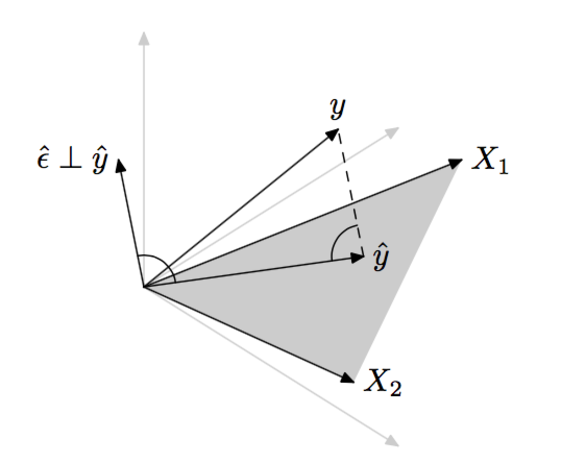
\includegraphics[width=4in]{img/olsGeom.pdf}
\end{center}

\end{frame}


%%%%%%%%%%%%%%%%%%%%%%%%%%%%%%%%%%%%%%%%%%%%%%%%%%%
\begin{frame}[fragile] \frametitle{}

{\bf Three final definitions}

The residuals, estimate of the $\sigma^2$ parameter,
and sum of squared residuals are given as:
\begin{align*}
r &= y - X\widehat{\beta} \\
s^2 &= \frac{1}{n-p} r^t r \\
\text{SSR} &= r^t r
\end{align*}

\end{frame}


%%%%%%%%%%%%%%%%%%%%%%%%%%%%%%%%%%%%%%%%%%%%%%%%%%%
\begin{frame}[fragile] \frametitle{}

\begin{center}
{\Large Classical linear model assumptions}
\end{center}

{\bf I. Linearity} $\quad Y = X\beta + \epsilon$

{\bf II. Strict exogeneity} $\quad \mathbb{E} \left( \epsilon | X \right) = 0$

{\bf III. No multicollinearity} $\quad \mathbb{P} \left[ \text{rank} (X) = p \right] = 1$

{\bf IV. Spherical errors} $\quad \mathbb{V} \left( \epsilon | X \right) = \sigma^2 \mathbb{I}_n$

{\bf V. Normality} $\quad \epsilon | X \sim \mathcal{N} (0, \sigma^2 \mathbb{I}_n)$

\end{frame}


%%%%%%%%%%%%%%%%%%%%%%%%%%%%%%%%%%%%%%%%%%%%%%%%%%%
\begin{frame}[fragile] \frametitle{}

{\bf Finite sample properties}

Under assumptions I-III:

\hspace{1cm} (A) $\mathbb{E} (\widehat{\beta} | X) = \beta$

Under assumptions I-IV:

\hspace{1cm}  (B)  $\mathbb{V} (\widehat{\beta} | X) = \sigma^2 (X^t X)^{-1}$

\hspace{1cm}  (C) $\widehat{\beta}$ is the best linear unbiased estimator (Gauss-Markov)

\hspace{1cm}  (D) $Cov( \widehat{\beta}, r | X) = 0$

\hspace{1cm}  (E) $\mathbb{E} (s^2 | X) = \sigma^2$

Under assumptions I-V:

\hspace{1cm}  (F) $\widehat{\beta}$ achieves the Cramér–Rao lower bound

\end{frame}

%%%%%%%%%%%%%%%%%%%%%%%%%%%%%%%%%%%%%%%%%%%%%%%%%%%
\begin{frame}[fragile] \frametitle{}

{\bf T-test}

Under assumptions $I-V$, to test the hypothesis that $H_0: \beta = b_j$
we construct the following T-test:
\begin{align*}
t &= \frac{\widehat{\beta}_j - b_j}{\sqrt{s^2  \left( (X^t X)^{-1}_{jj} \right)}} \\
&= \frac{\widehat{\beta}_j - b_j}{\text{S.E.}(\widehat{\beta}_j)} \\
&\sim t_{n-p}
\end{align*}

There is also a corrisponding confidence interval using the same standard
error.

\end{frame}

%%%%%%%%%%%%%%%%%%%%%%%%%%%%%%%%%%%%%%%%%%%%%%%%%%%
\begin{frame}[fragile] \frametitle{}

The Hypothesis test $H_0: D\beta = d$ for a full rank $k$ by $p$ matrix
$D$ yields the following {\bf F-test}:
\begin{align*}
F &= \frac{(\text{SSR}_R -  \text{SSR}_U) / k }{\text{SSR}_U / (n - p)}
\end{align*}
Where we let $\text{SSR}_U$ be the sum of squared residuals of the unrestricted
model ($r^t r$) and $\text{SSR}_R$ be the sum of squared residuals of the
restricted model (where the sum of squares is minimzed subject
to $D\beta = d$).

\end{frame}

%%%%%%%%%%%%%%%%%%%%%%%%%%%%%%%%%%%%%%%%%%%%%%%%%%%
\begin{frame}[fragile] \frametitle{}

We did a lot of matrix manipulations in the proofs of these
two results. The most important `big picture' results to
remember are:

\begin{itemize}
\item If $B$ is a symmetric idempotent matrix and
$u \sim \mathcal{N} (0, \mathbb{I}_n)$, then
$u^t B u \sim \chi^2_{\text{tr(B)}}$.
\item If $B$ is a symmetric idempotent matrix, then
all of $B$'s eigenvalues are $0$ or $1$. In terms of
the $Q^t \Lambda Q$ eigen-value decomposition, this
helps explain why we think of $P$ and $M$ as projection
matricies.
\end{itemize}

\end{frame}

%%%%%%%%%%%%%%%%%%%%%%%%%%%%%%%%%%%%%%%%%%%%%%%%%%%
\begin{frame}[fragile] \frametitle{}

\footnotesize

\begin{verbatim}
> out <- lm(Height ~ Father + Gender, data=h)
> summary(out)

Call:
lm(formula = Height ~ Father + Gender, data = h)

Residuals:
    Min      1Q  Median      3Q     Max
-9.3708 -1.4808  0.0192  1.5616  9.4153

Coefficients:
            Estimate Std. Error t value Pr(>|t|)
(Intercept) 34.46113    2.13628   16.13   <2e-16 ***
Father       0.42782    0.03079   13.90   <2e-16 ***
GenderM      5.17604    0.15211   34.03   <2e-16 ***
---
Signif. codes:  0 ‘***’ 0.001 ‘**’ 0.01 ‘*’ 0.05 ‘.’ 0.1 ‘ ’ 1

Residual standard error: 2.277 on 895 degrees of freedom
Multiple R-squared:  0.5971,  Adjusted R-squared:  0.5962
F-statistic: 663.2 on 2 and 895 DF,  p-value: < 2.2e-16
\end{verbatim}
\end{frame}

%%%%%%%%%%%%%%%%%%%%%%%%%%%%%%%%%%%%%%%%%%%%%%%%%%%
\begin{frame}[fragile] \frametitle{}

We formally defined leverage as the diagonal
elements of the projection matrix:
\begin{align*}
l_i &= P_{ii} \\
&= \left[ X (X^t X)^{-1} X^t \right]_{ii}
\end{align*}

\end{frame}

%%%%%%%%%%%%%%%%%%%%%%%%%%%%%%%%%%%%%%%%%%%%%%%%%%%
\begin{frame}[fragile] \frametitle{}

From here, this suggested that we construct the following
confidence interval for the mean of $y_{new}$:
\begin{align*}
\widehat{\mathbb{E}(y_{new} | X)} &\in X_{new} \widehat{\beta} \pm t_{n-p,1-\alpha/2} \cdot
\sqrt{s^2 X_{new} (X^t X)^{-1} X_{new}^t} \\
\end{align*}

\end{frame}

%%%%%%%%%%%%%%%%%%%%%%%%%%%%%%%%%%%%%%%%%%%%%%%%%%%
\begin{frame}[fragile] \frametitle{}

Finally, we then constructed the following prediction interval:
\begin{align*}
y_{new} | X &\in X_{new} \widehat{\beta} \pm t_{n-p,1-\alpha/2} \cdot
\sqrt{s^2 \left[ I_k + X_{new} (X^t X)^{-1} X_{new}^t \right]} \\
\end{align*}
Which is exactly a factor of $s$ wider than the confidence interval.

\end{frame}


\end{document}











